\chapter{อัตราส่วนตรีโกณมิติพื้นฐาน}

\section{สามเหลี่ยมมุมฉาก}

\subsection{ส่วนประกอบของสามเหลี่ยมมุมฉาก}

สามเหลี่ยมมุมฉากเป็นสามเหลี่ยมที่มีมุมหนึ่งเป็นมุมฉาก หรือมีขนาด \(90^\circ\)

\begin{itemize}
	\item \(AB\) เป็น \textbf{ด้านตรงข้ามมุมฉาก} ซึ่งเป็นด้านที่ยาวที่สุดของสามเหลี่ยม
	\item \(BC\) เป็น \textbf{ด้านตรงข้ามมุม} \(A\)
	\item \(AC\) เป็น \textbf{ด้านประชิดมุม} \(A\)
\end{itemize}

\section{อัตราส่วนตรีโกณมิติพื้นฐาน}

\subsection{ไซน์ โคไซน์ และแทนเจนต์}

พิจารณาสามเหลี่ยมมุมฉาก \(ABC\) ซึ่งมีมุม \(C\) เป็นมุมฉาก 
โดยกำหนดให้ความยาวด้านตรงข้ามมุม \(A\),
ด้านประชิดมุม \(A\) และด้านตรงข้ามมุมฉาก
เป็น \(a\), \(b\) และ \(c\) หน่วย ตามลำดับ 


\begin{remarkbox}
	\begin{enumerate}
		\item \textbf{ไซน์ของมุม $A$} แทนด้วยสัญลักษณ์ $\sin(A)$ นิยามโดย
		\[
		\sin(A)=\frac{\text{ความยาวด้านที่อยู่ตรงข้ามมุม } A}{\text{ความยาวด้านตรงข้ามมุมฉาก}}
		=\frac{a}{c}
		\]
		
		\item \textbf{โคไซน์ของมุม $A$} แทนด้วยสัญลักษณ์ $\cos(A)$ นิยามโดย
		\[
		\cos(A)=\frac{\text{ความยาวด้านประชิดมุม } A}{\text{ความยาวด้านตรงข้ามมุมฉาก}}
		=\frac{b}{c}
		\]
		
		\item \textbf{แทนเจนต์ของมุม $A$} แทนด้วยสัญลักษณ์ $\tan(A)$ นิยามโดย
		\[
		\tan(A)=\frac{\text{ความยาวด้านที่อยู่ตรงข้ามมุม } A}{\text{ความยาวด้านประชิดมุม } A}
		=\frac{a}{b}
		\]
	\end{enumerate}
\end{remarkbox}


\begin{examplebox}
	พิจารณาสามเหลี่ยมมุมฉาก \(ABC\) โดยที่มุม \(C\) เป็นมุมฉาก และมุม \(A = 30^\circ\)
	
	ถ้าด้าน \(BC = 3\) หน่วย จงหาความยาวของด้าน \(AB\) และ \(AC\) โดยใช้อัตราส่วนตรีโกณมิติพื้นฐาน
\end{examplebox}

\begin{figure}[H] 
	\centering 
	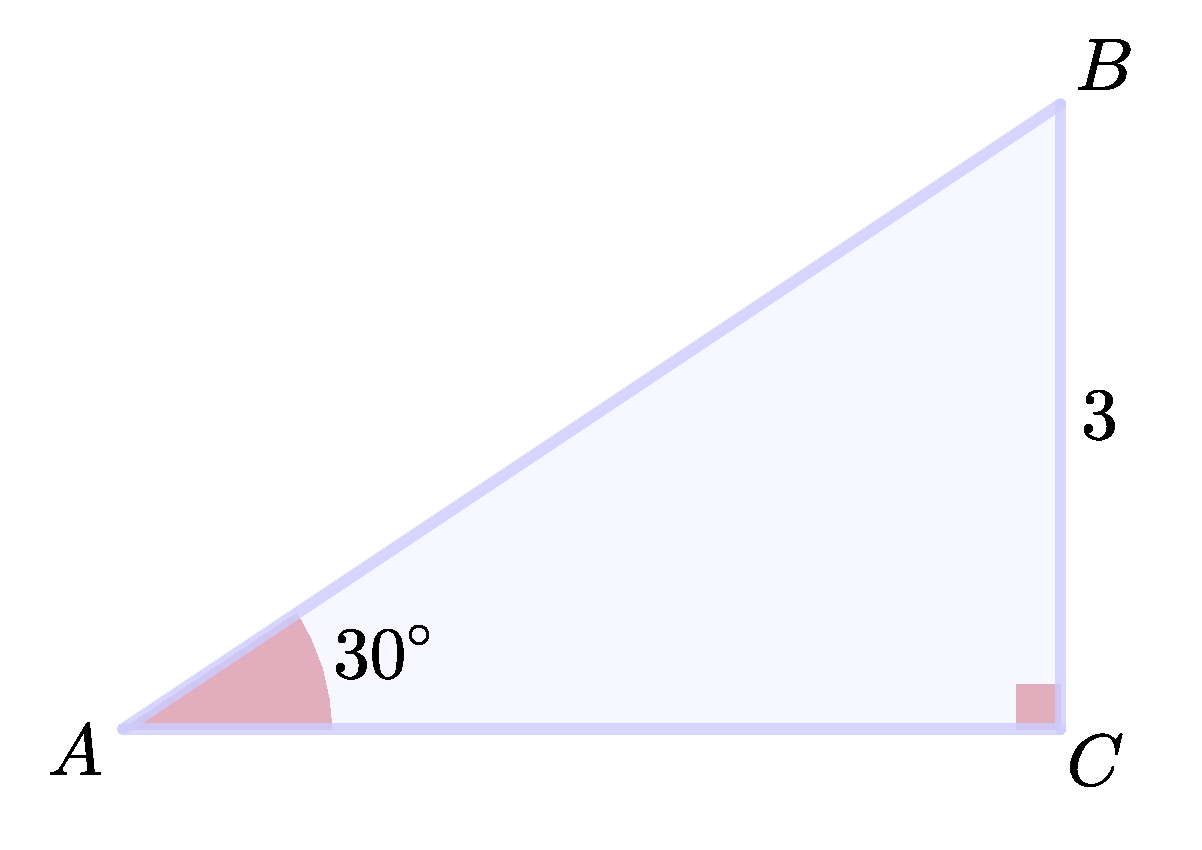
\includegraphics[scale=0.5]{3} 
	\caption{} 
	\label{Figure3} 
\end{figure}
\solution ตัวอย่างต่อไปนี้เป็นตัวอย่างเพิ่มเติมสำหรับฝึกการประยุกต์ใช้อัตราส่วนตรีโกณมิติในการหาความยาวด้านของสามเหลี่ยมมุมฉาก

\begin{examplebox}
	พิจารณาสามเหลี่ยมมุมฉาก \(ABC\) และ \(DBC\) ซึ่งทั้งสองสามเหลี่ยมมีมุมฉากที่จุด \(C\)
	
	ถ้ามุม \(A\) และ \(D\) มีขนาด \(30^\circ\) และ \(60^\circ\) ตามลำดับ และความยาวของด้าน \(BC\) เท่ากับ \(10\sqrt{3}\) หน่วย
	
	จงหาความยาวของด้าน \(AD\) โดยใช้อัตราส่วนตรีโกณมิติพื้นฐาน
\end{examplebox}
	\begin{figure}[H] 
		\centering 
		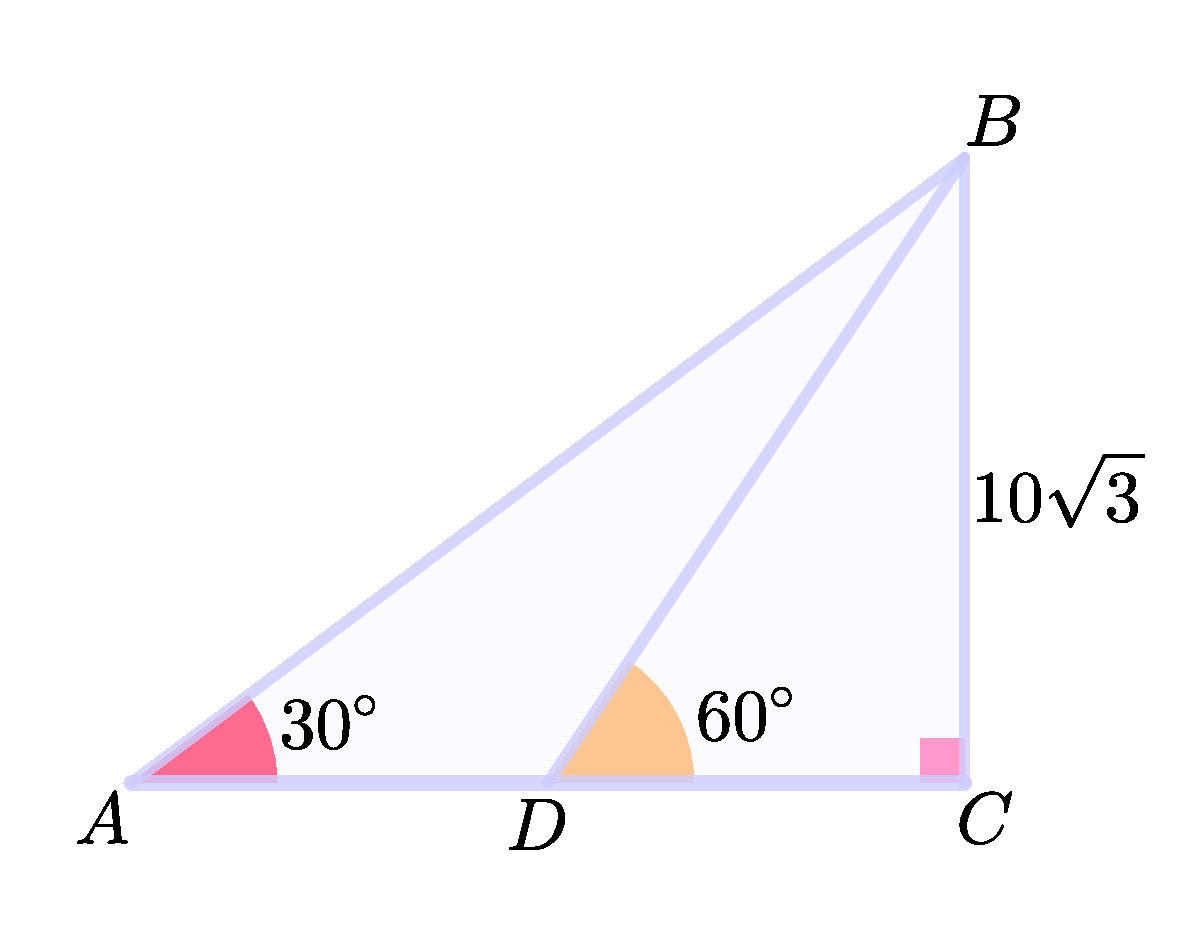
\includegraphics[scale=0.55]{4} 
		\caption{} 
		\label{Figure4} 
	\end{figure}
	\begin{solution}
		กำหนดให้ $x + 5 = 10$ \\
		จะได้ว่า $x = 10 - 5$ \\
		ดังนั้น $x = 5$
	\end{solution}

\begin{examplebox}\label{example2.1}
	\begin{align*}
		\{1,2,3\} \cup \{2,3,4\} &= \{1,2,3,4\}\\
		\{3,5\} \cup \{2,3,5\} &= \{2,3,5\}\\
		\{1,3,5\} \cup \{2,4,6\} &= \{1,2,3,4,5,6\} \\
		\{1,2\} \cup \varnothing &= \{1,2\}
	\end{align*}
\end{examplebox}

จากตัวอย่าง~\ref{example2.1} จะได้สมบัติที่สำคัญคือ  
\[
A \cup \varnothing = A 
\quad \text{และ} \quad 
A \cup \mathcal{U} = \mathcal{U}
\]

\begin{remarkbox}[หลักการรวมเข้า–เอาออก]
	ให้ $A,B$ และ $C$ เป็นเซตจำกัด โดยมีจำนวนสมาชิกเท่ากับ $n(A), n(B)$ และ $n(C)$ ตามลำดับ
	\begin{itemize}
		\item $n(A\cup B)=n(A)+n(B)-n(A\cap B)$
		\item $n(A\cup B\cup C)=n(A)+n(B)+n(C)-n(A\cap B)-n(B\cap C)-n(C\cap A)+n(A\cap B\cap C)$
	\end{itemize}
\end{remarkbox}